\documentclass[border=4pt]{standalone}
\usepackage{fontspec}
\usepackage{amsmath}
\usepackage{unicode-math}
\setmainfont{Latin Modern Roman}
\setmathfont{Latin Modern Math}
\usepackage{pgfplots}
\usepackage{pgfplotstable}
\pgfplotsset{compat=1.18}
\usepackage{tkz-euclide}
\usetikzlibrary{arrows.meta,calc,angles,quotes,patterns,3d,backgrounds}
\definecolor{ink}{HTML}{123428}
\definecolor{asy}{HTML}{475569}
\definecolor{mint}{HTML}{86e0bd}
\tikzset{asym/.style={asy, line width=0.9pt, dash pattern=on 5pt off 3.5pt},
         guide/.style={gray!70, line width=0.6pt, densely dotted},
         dot/.style={circle, inner sep=0pt, minimum size=5pt, draw=white, line width=0.5pt},
         odot/.style={circle, inner sep=0pt, minimum size=5.5pt, fill=white, line width=1pt},
         lab/.style={font=\footnotesize, inner sep=1.5pt, text=ink}}
\begin{document}
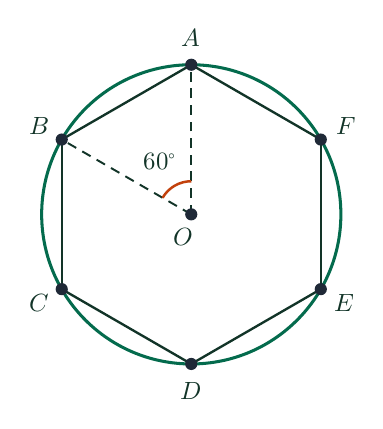
\begin{tikzpicture}
\draw[color={rgb,255:red,4;green,107;blue,77}, line width=1.1pt] (0,0) circle (1.900);
\draw[ink, line width=0.85pt] (0.000,1.900) -- (-1.645,0.950);
\draw[ink, line width=0.85pt] (-1.645,0.950) -- (-1.645,-0.950);
\draw[ink, line width=0.85pt] (-1.645,-0.950) -- (-0.000,-1.900);
\draw[ink, line width=0.85pt] (-0.000,-1.900) -- (1.645,-0.950);
\draw[ink, line width=0.85pt] (1.645,-0.950) -- (1.645,0.950);
\draw[ink, line width=0.85pt] (1.645,0.950) -- (0.000,1.900);
\draw[ink, line width=0.7pt, dash pattern=on 3.5pt off 2.5pt] (0.000,0.000) -- (0.000,1.900);
\draw[ink, line width=0.7pt, dash pattern=on 3.5pt off 2.5pt] (0.000,0.000) -- (-1.645,0.950);
\draw[color={rgb,255:red,194;green,65;blue,12}, line width=0.9pt] (0.000,0.420) -- (-0.022,0.419) -- (-0.044,0.418) -- (-0.066,0.415) -- (-0.087,0.411) -- (-0.109,0.406) -- (-0.130,0.399) -- (-0.151,0.392) -- (-0.171,0.384) -- (-0.191,0.374) -- (-0.210,0.364) -- (-0.229,0.352) -- (-0.247,0.340) -- (-0.264,0.326) -- (-0.281,0.312) -- (-0.297,0.297) -- (-0.312,0.281) -- (-0.326,0.264) -- (-0.340,0.247) -- (-0.352,0.229) -- (-0.364,0.210);
\node[font=\small, text=ink, inner sep=0.5pt, fill=white] at (-0.390,0.675) {$60^\circ$};
\fill[color={rgb,255:red,31;green,41;blue,55}] (0.000,1.900) circle (2.2pt);
\fill[color={rgb,255:red,31;green,41;blue,55}] (-1.645,0.950) circle (2.2pt);
\fill[color={rgb,255:red,31;green,41;blue,55}] (-1.645,-0.950) circle (2.2pt);
\fill[color={rgb,255:red,31;green,41;blue,55}] (-0.000,-1.900) circle (2.2pt);
\fill[color={rgb,255:red,31;green,41;blue,55}] (1.645,-0.950) circle (2.2pt);
\fill[color={rgb,255:red,31;green,41;blue,55}] (1.645,0.950) circle (2.2pt);
\fill[color={rgb,255:red,31;green,41;blue,55}] (0.000,0.000) circle (2.2pt);
\node[font=\small, text=ink, inner sep=0.5pt] at (0.000,2.240) {$A$};
\node[font=\small, text=ink, inner sep=0.5pt] at (-1.940,1.120) {$B$};
\node[font=\small, text=ink, inner sep=0.5pt] at (-1.940,-1.120) {$C$};
\node[font=\small, text=ink, inner sep=0.5pt] at (-0.000,-2.240) {$D$};
\node[font=\small, text=ink, inner sep=0.5pt] at (1.940,-1.120) {$E$};
\node[font=\small, text=ink, inner sep=0.5pt] at (1.940,1.120) {$F$};
\node[font=\small, text=ink, inner sep=0.5pt] at (-0.103,-0.282) {$O$};
\end{tikzpicture}
\end{document}
